\chapter{Data and Methods}\label{sec:data_methods}
{
	We will start by describing the available data and the challenges associated with it.
	Our study region is a farm of over 800ha, which is located in western Switzerland. From \cite{perichPixelbasedCropYield2022}  we acquire satellite image data (section \ref{sec:s2_img_data}), yield maps of several cereals from 2017 to 2021 (section \ref{sec:yieldmapping_data}), and meteorological data (section \ref{sec:gather_data_to_pixel}).
	Afterwards, we will introduce general methods in section \ref{sec:general_methods}, which will be used in the remaining chapters.
}


\section{Sentinel 2 Data}{
	\label{sec:s2_img_data}
	%\subsection*{General Information}
	{
		% wie zitiere ich diese url's am besten? BibTex schlägt fehl, da der Autor-name nicht eindeutig ist ('die ESA'?)
		The European Space Agency \citep{esaSentinel22022} freely distributes the high-quality images of the two Sentinel satellites (S2). Together, both satellites have a revisit time of 5 days at the Equator and 2-3 days at mid-latitudes. However, in our study region, we only receive an image every 5 days.
		
		\begin{table}[h]
    \centering
    \small
    \caption{List of spectral bands of the S2-satellites. Each band has its center at the wavelength $\lambda$ in $nm$ with the spectral width $\Delta\lambda$ in $nm$ with a spatial resolution $SR$ in $m$ \citep{jaramazESASentinel2Mission2013}.}
    \begin{tabular}{p{0.03\linewidth} p{0.04\linewidth} p{0.03\linewidth} p{0.03\linewidth} p{0.73\linewidth}}
    \toprule
        \hspace*{-5pt} Band & $\;\lambda$ & $\Delta\lambda$ & $SR$ & Purpose \\ \hline
        1 & 443 & 20 & 60 & Atmospheric correction (aerosol scattering) \\ %\hline
        2 & 490 & 65 & 10 & Sensitive to vegetation senescing, carotenoid, browning and soil background; atmospheric correction (aerosol scattering) \\ %\hline
        3 & 560 & 35 & 10 & Green peak, sensitive to total chlorophyll in vegetation \\ %\hline
        4 & 665 & 30 & 10 & Maximum chlorophyll absorption \\ %\hline
        5 & 705 & 15 & 20 & Position of red edge; consolidation of atmospheric corrections / fluorescence baseline. \\ %\hline
        6 & 740 & 15 & 20 & Position of red edge, atmospheric correction, retrieval of aerosol load. \\ %\hline
        7 & 783 & 20 & 20 & Leaf Area Index (LAI), edge of the Near-Infrared (NIR) plateau. \\ %\hline
        8 & 842 & 115 & 10 & LAI \\ %\hline
        8a & 865 & 20 & 20 & NIR plateau, sensitive to total chlorophyll, biomass, LAI and protein; water vapor absorption reference; retrieval of aerosol load and type. \\ %\hline
        9 & 945 & 20 & 60 & Water vapor absorption, atmospheric correction. \\ %\hline
        10 & 1375 & 30 & 60 & Detection of thin cirrus for atmospheric correction. \\ %\hline
        11 & 1610 & 90 & 20 & Sensitive to lignin, starch and forest above ground biomass. Snow/ice/cloud separation. \\ %\hline
        12 & 2190 & 180 & 20 & Assessment of Mediterranean vegetation conditions. Distinction of clay soils for the monitoring of soil erosion. Distinction between live biomass, dead biomass and soil, e.g., for burn scars mapping. \\
        \bottomrule
    \end{tabular}
    \label{table:S2-bands}
\end{table}

		
		The S2 images contain 12 spectral bands with spatial resolutions up to 10 meters (see \ref{table:S2-bands}). Bands with a lower resolution (20 and 60 meters) were upscaled to 10 meter resolution using cubic interpolation \citep{perichPixelbasedCropYield2022}. In order to decrease the effect of atmospheric conditions like reflections and scattering, bottom-of-atmosphere, radiometric corrected Level-2A data was used\footnote{According to \cite{perichPixelbasedCropYield2022}: ``Data prior to March 2018 was only available in the top-of-atmosphere L1C format and was downloaded as such [...] L1C data was processed to L2A product level using the `Sen2Cor' processor provided by the European Space Agency''}. 
		The European Space Agency also supplies an algorithm \citep{esaLevel2AAlgorithmOverview2022} produces Scene Classification Layer ({SCL}) where for each location the observed subject is assigned to one of 11 SCL-classes (cf. table~\ref{tab:satelite/scl_classes}). 
		In this thesis,  we will use this classification to filter out data points, that we belive to be less informative. That are all observations which SCL-class does not correspond to vegetation or bare soils (classes 4 and 5). For convenience, we define the set SCL45 as the observations that belong to SCL-class 4 or 5.
		
		% \begin{figure}[h]
		% 	\label{fig:satelite/sentinel-2-bands}
		% 	\center
		% 	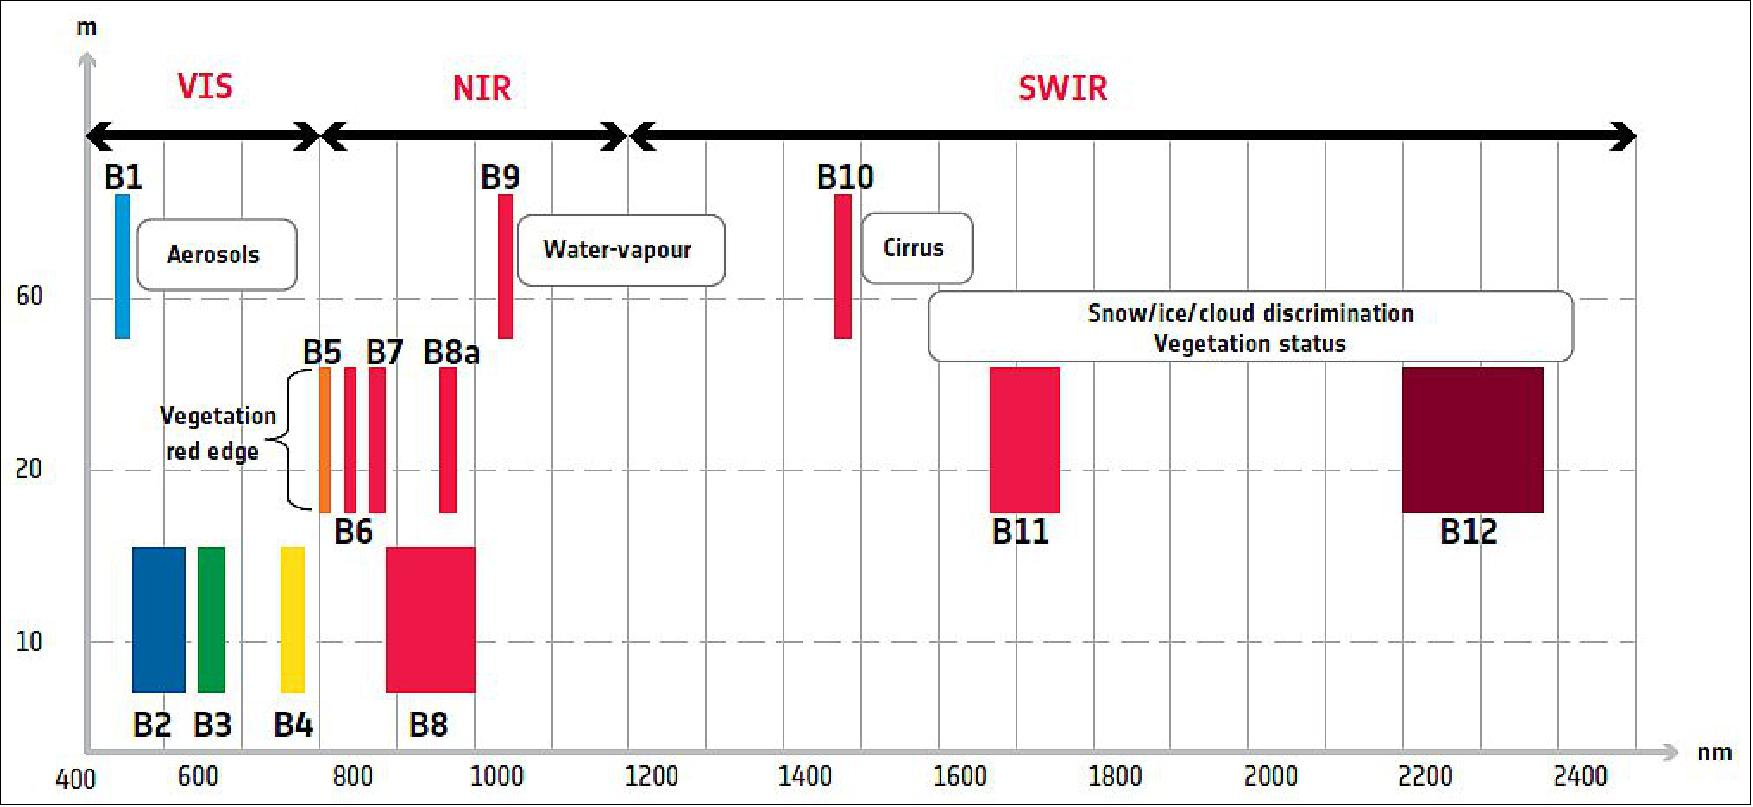
\includegraphics[width=0.4\textwidth]{satelite/sentinel-2-bands.jpg}
		% 	\caption{XXX Sentinel 2 bands}
		% \end{figure}
				% \begin{table}[!h]
		% 	\caption{Overview: Scene Classification Layers (SCL)}
		% 	\label{tab:satelite/scl_classes}
		% 	\center
		% 	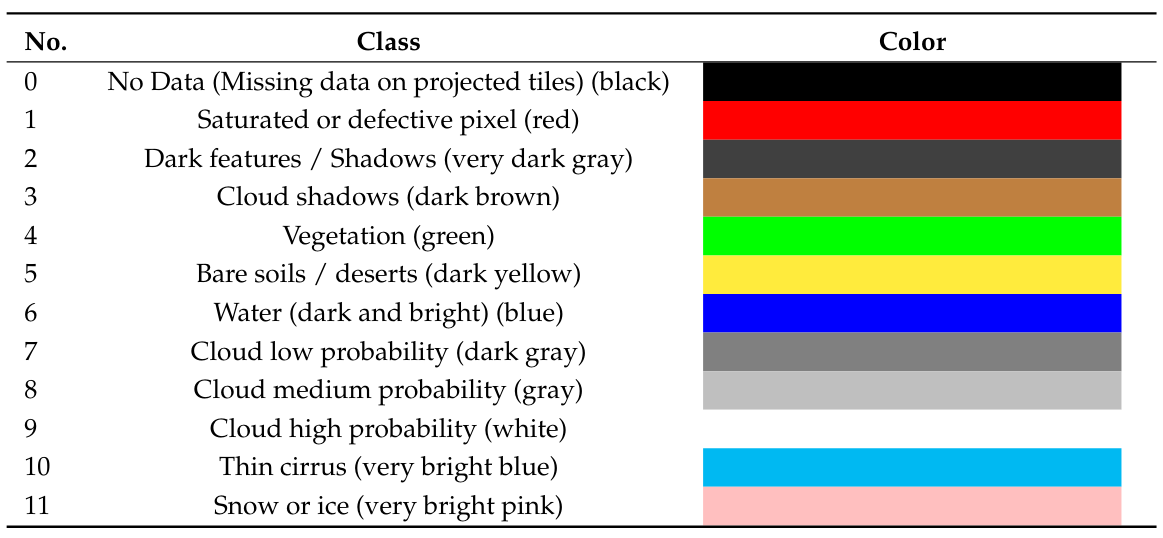
\includegraphics[width=0.8\textwidth]{satelite/scl_classes.png}
		% \end{table}
		
		\begin{table}[h]
			\caption{Overview: Scene Classification Layers (SCL)}
			\label{tab:satelite/scl_classes}
			\centering
			\small
			\begin{tblr}{
			  colspec = {p{0.05\linewidth} p{0.03\linewidth} p{0.3\linewidth} p{0.05\linewidth} p{0.03\linewidth} p{0.3\linewidth} },
			%   row{2} = {SCL3color},
			%   column{3} = {teal7},
			  cell{2}{1} = {SCL0color},
			  cell{3}{1} = {SCL1color},
			  cell{4}{1} = {SCL2color},
			  cell{5}{1} = {SCL3color},
			  cell{6}{1} = {SCL4color},
			  cell{7}{1} = {SCL5color},
			  cell{2}{4} = {SCL6color},
			  cell{3}{4} = {SCL7color},
			  cell{4}{4} = {SCL8color},
			  cell{5}{4} = {SCL9color},
			  cell{6}{4} = {SCL10color},
			  cell{7}{4} = {SCL11color},
			}
			% \toprule % not working :8
			\hline
			Color & No. & Class & Color & No. & Class \\
			\hline
			& 0: & Missing Data 	& & 6: &  Water\\	 
			& 1: & Saturated or defective pixel 	& & 7: &  Cloud low probability\\
			& 2: & Dark features / Shadows 	& & 8: &  Cloud medium probability\\
			& 3: & Cloud shadows 	& & 9: &  Cloud high probability\\
			& 4: & Vegetation 	& & 10: &  Thin cirrus cloud\\
			& 5: & Bare soils 	& & 11: &  Snow or ice\\
			  \hline
			%   \bottomrule
			\end{tblr}
		  \end{table}


	% 0: "#000000",  Missing Data
	% 1: "#ff0000",	 Saturated or defective pixel
	% 2: "#404040",  Dark features / Shadows
	% 3: "#bf8144",  Cloud shadows
	% 4: "#00ff3c",  Vegetation
	% 5: "#ffed50",  Bare soils
	% 6: "#0d00fa",  Water
	% 7: "#808080",  Cloud low probability
	% 8: "#bfbfbf",  Cloud medium probability
	% 9: "#eeeeee",  Cloud high probability
	% 10: "#0bb8f0", Thin cirrus cloud
	% 11: "#ffbfbf", Snow or ice

		

	}
}

\section{Crop Yield Data}{
	\label{sec:yieldmapping_data}
	The crop yield data were collected using a combine harvester. Equipped with GPS, the harvester drives over the fields and continuously estimates the dry crop yield density in $t/ha$ (see fig. \ref{fig:satelite/witzwil_2021_P112_yield_harvester_cropped}). 
	We take the data set derived in \cite{perichPixelbasedCropYield2022}, where error-prone measurement points (such as during a tight curve of the combine harvester) were removed and then the yield map was rasterized using linear interpolation (cf. fig. \ref{fig:satelite/witzwil_2021_P112_yield_cropped.png}). We summarize the rasterized dry-yield values by the following statistics:

	% tabelle anstadt histogramm, da schon zu viele figuren ``herumschwirren'' und es so kompakter ist.
	\begin{tabular}{l l l l l l l} 
		Minimum & 1st Quartile & Median & Mean  & 3rd Quartile & Maximum & Variance \\
		0.107   & 6.186        & 7.560  & 7.359 & 8.756        & 13.35   & 4.035
	\end{tabular}    

	Comparing the average per-field crop yield reported by the farmer with the yield estimated by the combine harvester shows that the latter overestimates crop yield by ca. $10\%$ \citep{perichPixelbasedCropYield2022}. Since the relative estimation error is approximately constant and we do not aim for an accurate yield prediction, we will not consider this deviation. 



	\begin{figure}
		\centering
		\begin{subfigure}{.5\textwidth}
			\centering
			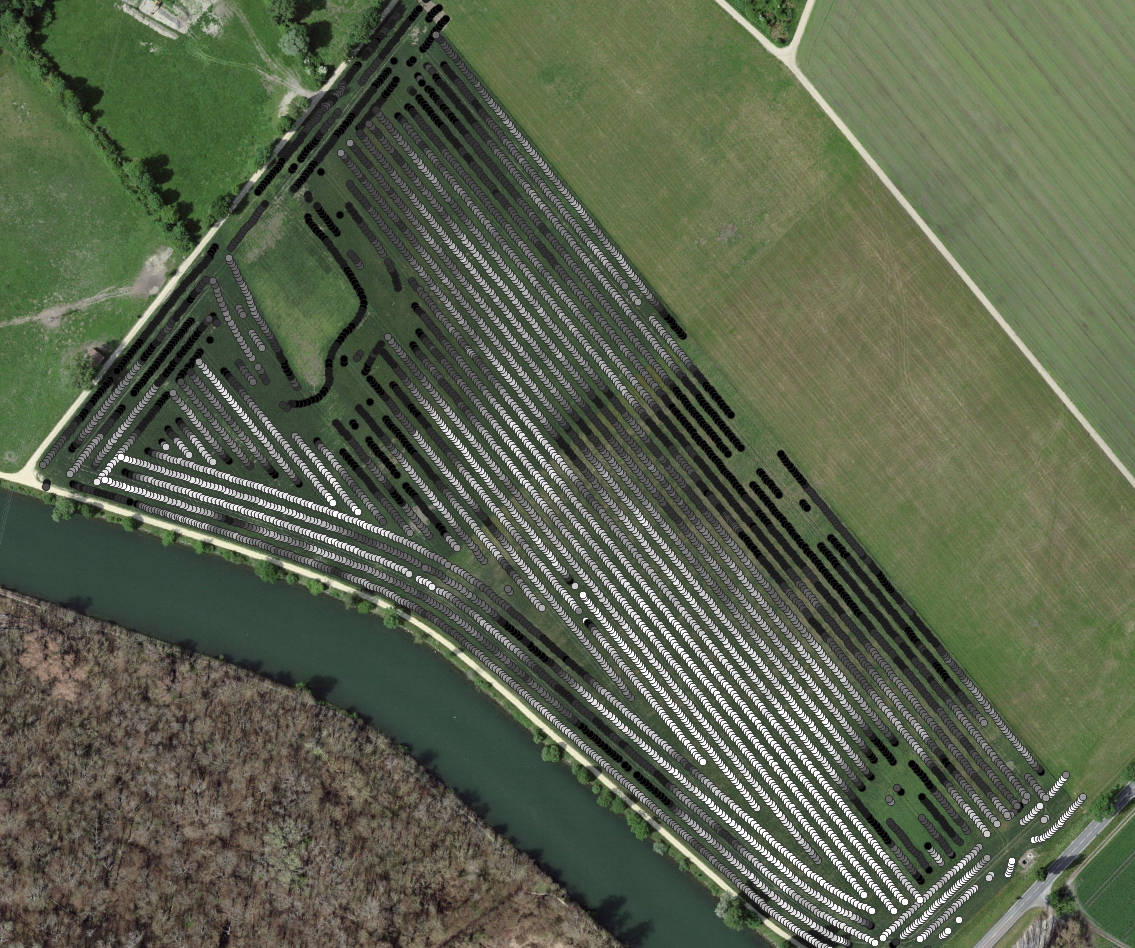
\includegraphics[height=.75\linewidth]{satelite/witzwil_2021_P112_yield_harvester_cropped.png}
			\caption{Raw combine harvester data (cleaned)}
			\label{fig:satelite/witzwil_2021_P112_yield_harvester_cropped}
		\end{subfigure}%
		\begin{subfigure}{.5\textwidth}
			\centering
			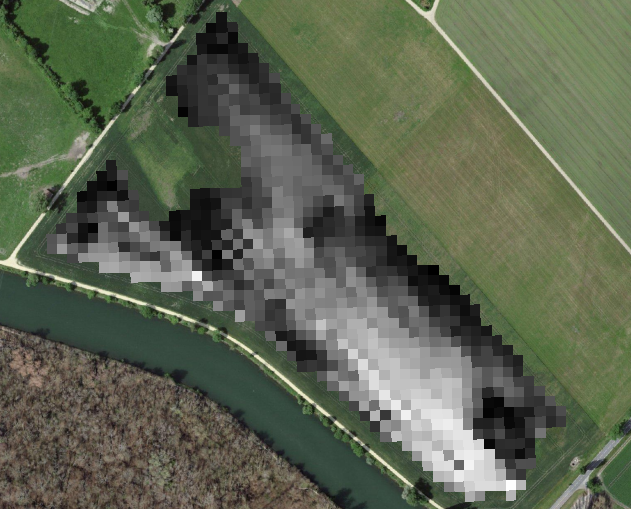
\includegraphics[height=.75\linewidth]{satelite/witzwil_2021_P112_yield_cropped.png}
			\caption{rasterized to Sentinel 2 resolution.}
			\label{fig:satelite/witzwil_2021_P112_yield_cropped.png}
		\end{subfigure}
		\caption{Crop yield density map of a field. Ranges from 0.1 t/ha (black) to 5.35 t/ha (white) }
		\label{fig:satelite_witzwil_yield}
	\end{figure}

}

\section{Normalized Difference Vegetation Index (NDVI)}{% NDVI
	The well-known  ({NDVI}) introduced in \cite{rouseMonitoringVernalAdvancement1974} is used to measure vegetation in remote sensing. It utilizes a large jump of reflectancy between red and infrared and can be calculated using the bands $B4$ and $B8$ (table \ref{table:S2-bands}) by:
	\begin{equation}
		NDVI = \frac{B8 - B4}{B8 + B4}
		\label{eq:ndvi}
	\end{equation}
	Since we measure the NDVI via the S2 satelites from space we can not expect to measure the true NDVI. This is especially true if we do not see the ground because of clouds or the ground signal is disturbed by cloud shadows. Even if we only use SCL45 observations we still encouter issues as will be described in section \ref{sec:s2_challangges}. Therefore, we call the calculated values merely the {observed NDVI}. In the following chapters, we will study the resulting NDVI {TS} (for one location and one season) extensively. Such a {TS} is shown in figure \ref{interpol/ndvi_ts_das_grey.pdf}.
	\begin{figure}[!h]
		\centering
		\begin{subfigure}{.47\textwidth}
			% \centering
			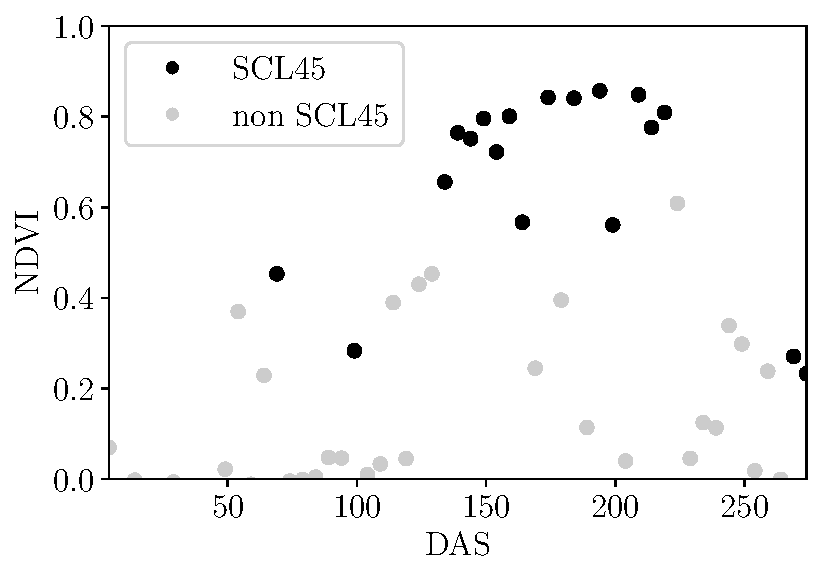
\includegraphics[height=.75\linewidth]{interpol/ndvi_ts_das_grey.pdf}
			\caption{Days After Sowing (DAS)}
			\label{interpol/ndvi_ts_das_grey.pdf}
		\end{subfigure}%
		\hfill
		\begin{subfigure}{.47\textwidth}
			% \centering
			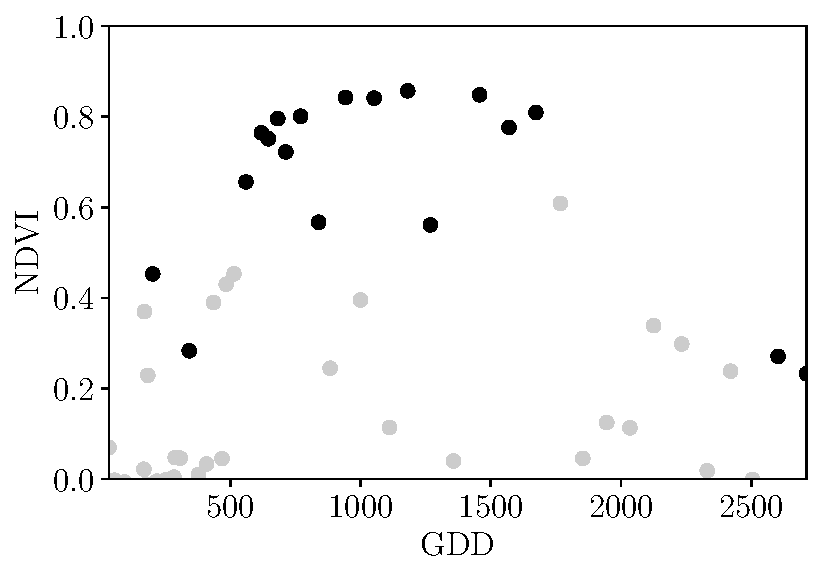
\includegraphics[height=.75\linewidth]{interpol/ndvi_ts_gdd_grey.pdf}
			\caption{Growing Degree Days (GDD)}
			\label{interpol/ndvi_ts_gdd_grey.pdf}
		\end{subfigure}
		\caption{NDVI {TS} plotted against DAS and GDD. GDD are introduced in section \ref{sec:gdd_def}.}
		\label{fig:raw_ndvi_ts}
	\end{figure}
}
% \section{DAS vs. GDD}{
% %example plot
% Prior to interpolating the NDVI {TS}, we should decide on a timescale. We can choose between DAS and GDD\todo{Findet man hier noch Literatur, in welcher ähnliches diskutiert wurde, die man zitieren kann?} (cf. section \ref{sec:gather_data_to_pixel} and equation \refeq{eq:gdd}). 
% This has several advantages. First, it makes the scales comparable (in terms of plant growth) because the plants are not concerned with the month of the year but the current temperature. Second, in winter we tend to have higher cloud cover and thus fewer SCL45 observations. 

% \begin{my_figure}[h]{width=0.8\textwidth}{interpol/das_vs_gdd}
% 	\caption{The same NDVI time-series, on the left with DAS as the timescale, on the right GDD is the timescale. SCL45 are colored black. Non-SCL45 (clouds and shadows) are colored in gray.}
% 	\label{fig:interpol/das_vs_gdd}
% \end{my_figure}
\section{Timescale Transformation}\label{sec:gdd_def}
	{% GDD & DAS
		Regarding the Days After Sowing (DAS) time scale shown in fig. \ref{interpol/ndvi_ts_das_grey.pdf}, we detect two drawbacks. First, this scale makes it difficult to compare two NDVI {TS} because wheat is not always sown on the same day of the year and in some years plants begin to emerge earlier. Second, because there are only few SCL45 observations in the winter, we face significant data gaps in this period. The time scale transformation introduced in \cite{mcmasterGrowingDegreedaysOne1997} fixes both problems. The resulting Growing Degree Days ({GDD}) are defined as the cumulative sum since sowing of temperature above a given base temperature $T_{base}$. For cereals, we use $T_{base}=0$ \citep{perichPixelbasedCropYield2022}. Thus, the GGD for $n$ days after sowing will be equal to:
		\begin{equation}
			\label{eq:gdd}
			GDD_n := \sum_{i=0}^n \max(T_i - T_{base}, 0).
		\end{equation}
		Important plant growth stages and their corresponding GDD values are tabultaed in \ref{app:gdd_examples}

		In figure \ref{fig:raw_ndvi_ts} we see an example for comparison of the DAS and GDD timescale. Here we see that the first 120 DAS are compressed to just 500 GDD and hence the gap in observations was succesfully compressed. Due to the reasons mentioned above, from now on we will only consider GDD.
	} 

\section{The Concept of a `Pixel'}{ \label{sec:gather_data_to_pixel}
	Now we create a new data structure that we call Pixel. This originates from the pixels of the S2 satellite images. It will contain all the information needed to confront the tasks in the following chapters. 
		
		Consider a 10 by 10 meter square that coinsides with a S2 image pixel and $T$ the GDD values for which S2 images are avialable in a given season. For $t\in T$ let $P_t$ be a tupel of all the spectral bands, the observed NDVI and the SCL class (at the considered location at time $t$). Then, define $P$ as the collection of all the $P_t$ and the estimated dry-yield for this square.
		Analogously to $P$, define $P^{SCL45}$ by only considering $P_t$ with SCL-class 4 or 5 (vegetation and soil).  
}

		% We will call the resulting data set {PIXELS}, as it is the collection of all Pixels (over all seasons). 
		
		% Finally, we split PIXELS randomly into a train ($80\%$) and test  ($20\%$) set. 
\section{Challenges in S2 Data}{\label{sec:s2_challangges}
		%satelite/time_series_2021_P112/15_scl5_2021-02-23.png
	%satelite/time_series_2021_P112/30_scl4_2021-05-09.png
	%satelite/time_series_2021_P112/33_scl9_2021-05-24.png
	%satelite/time_series_2021_P112/35_scl4_2021-06-03.png
	%satelite/time_series_2021_P112/40_scl10_2021-06-28.png
	%satelite/time_series_2021_P112/45_scl2_2021-07-23.png

\begin{figure*}
	\centering
	\begin{subfigure}[b]{0.31\textwidth}
		\centering
		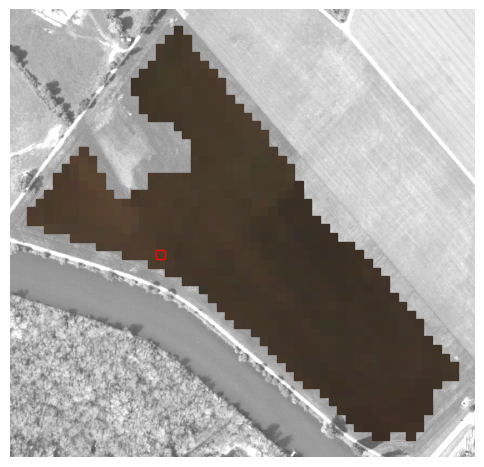
\includegraphics[width=\textwidth]{satelite/time_series_2021_P112/15_scl5_2021-02-23.png}
		\caption[2021-02-23\hspace*{0.1cm} SCL 5]%
		{{\small 2021-02-23\hspace*{0.1cm} SCL 5}}    
		\label{fig:satelite/time_series_2021_P112/15_scl5_2021-02-23.png}
	\end{subfigure}
	\hfill
	\begin{subfigure}[b]{0.31\textwidth}  
		\centering 
		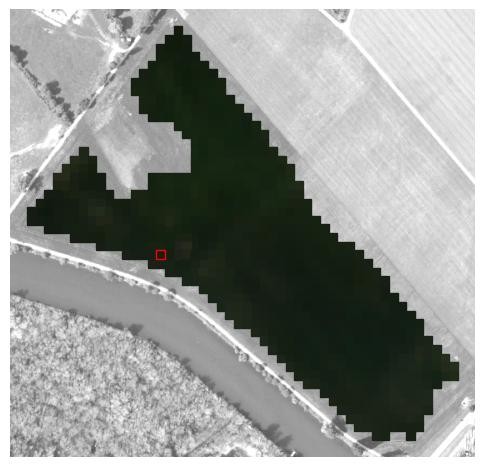
\includegraphics[width=\textwidth]{satelite/time_series_2021_P112/30_scl4_2021-05-09.png}
		\caption[2021-05-09\hspace*{0.1cm} SCL 4]%
		{{\small 2021-05-09\hspace*{0.1cm} SCL 4}}    
		\label{fig:satelite/time_series_2021_P112/30_scl4_2021-05-09.png}
	\end{subfigure}
	\hfill
	\begin{subfigure}[b]{0.31\textwidth}  
		\centering 
		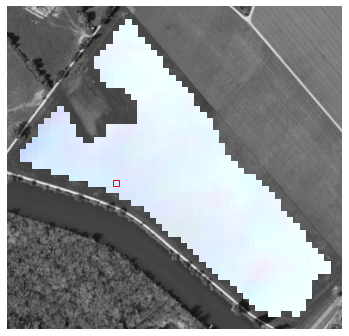
\includegraphics[width=\textwidth]{satelite/time_series_2021_P112/33_scl9_2021-05-24.png}
		\caption[2021-05-24\hspace*{0.1cm} SCL 9]%
		{{\small 2021-05-24\hspace*{0.1cm} SCL 9}}    
		\label{fig:satelite/time_series_2021_P112/33_scl9_2021-05-24.png}
	\end{subfigure}

	\vskip\baselineskip
	\begin{subfigure}[b]{0.31\textwidth}   
		\centering 
		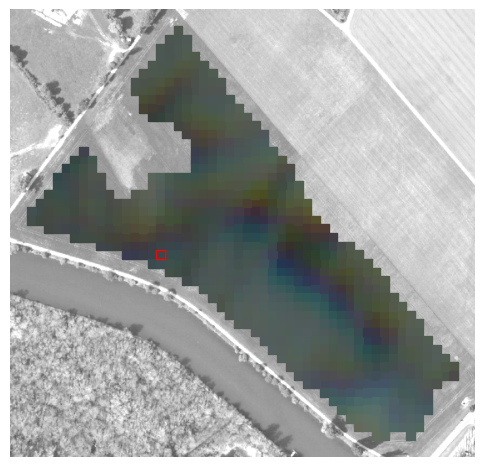
\includegraphics[width=\textwidth]{satelite/time_series_2021_P112/35_scl4_2021-06-03.png}
		\caption[2021-06-03\hspace*{0.1cm} SCL 4]%
		{{\small 2021-06-03\hspace*{0.1cm} SCL 4}}    
		\label{fig:satelite/time_series_2021_P112/35_scl4_2021-06-03.png}
	\end{subfigure}
	\hfill
	\begin{subfigure}[b]{0.31\textwidth}   
		\centering 
		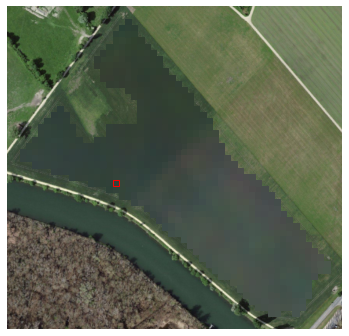
\includegraphics[width=\textwidth]{satelite/time_series_2021_P112/40_scl10_2021-06-28.png}
		\caption[2021-06-28\hspace*{0.1cm} SCL 10]%
		{\small 2021-06-28\hspace*{0.1cm} SCL 10}    
		\label{fig:satelite/time_series_2021_P112/40_scl10_2021-06-28.png}
	\end{subfigure}
	\hfill
	\begin{subfigure}[b]{0.31\textwidth}  
		\centering 
		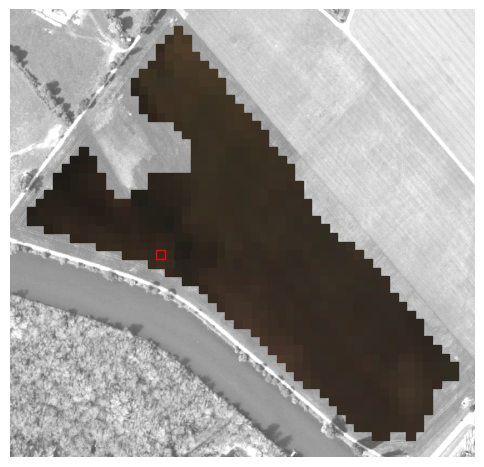
\includegraphics[width=\textwidth]{satelite/time_series_2021_P112/45_scl2_2021-07-23.png}
		\caption[2021-07-23\hspace*{0.1cm} SCL 2]%
		{{\small 2021-07-23\hspace*{0.1cm} SCL 2}}    
		\label{fig:satelite/time_series_2021_P112/45_scl2_2021-07-23.png}
	\end{subfigure}

	\vskip\baselineskip
	\begin{subfigure}[b]{0.7\textwidth}   
		\centering 
		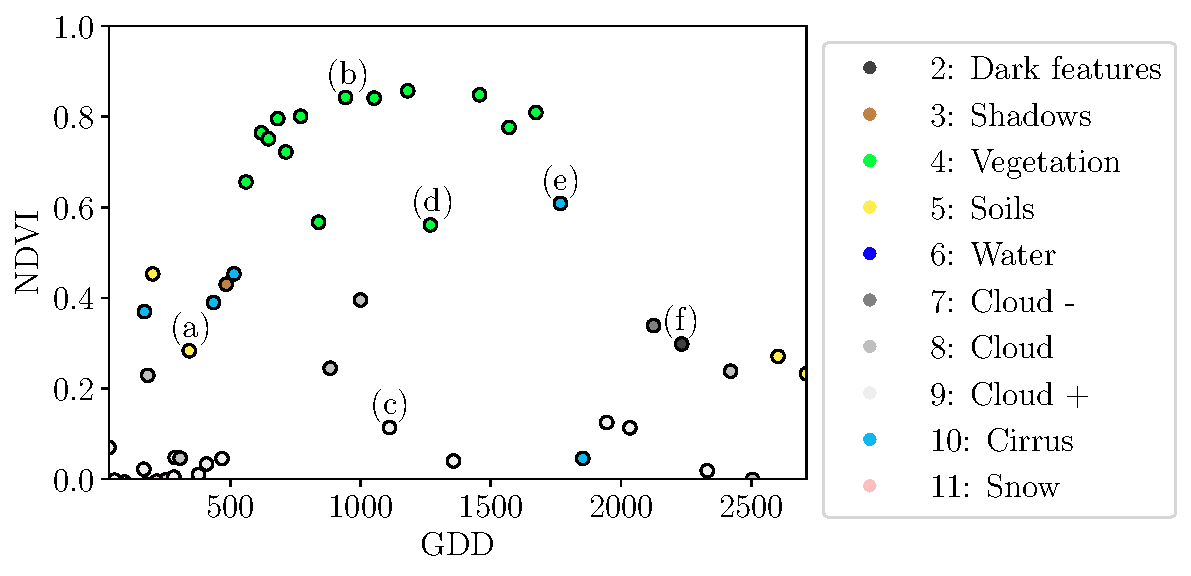
\includegraphics[width=\textwidth]{interpol/ndvi_ts_scl.pdf}
		\caption[Corresponding NDVI {TS}]%
		{{\small Corresponding NDVI {TS}}}    
		\label{fig:interpol/ndvi_ts_scl45_grey.pdf}
	\end{subfigure}
	\vspace{0.3cm}
	\caption[Satellite images of a field at selected times + NDVI TS]{Satellite images of a field at selected times with a static grayscale background for orientation. Moreover, the NDVI {TS} of the red-highlighted pixel is shown in (g) colored by the SCL labels.} 
	\label{fig:witzwil_selected_satellite_images}
\end{figure*}



	% Description of plot
	Now, we shall illustrate with an example pixel the challenges, we will confront in the coming chapters. The figure~\ref{fig:witzwil_selected_satellite_images} shows a selection of 6 satellite images of a field, one selected Pixel and the NDVI {TS} of this pixel. 		
	In February (image a), we see no vegetation but bare soil and thus also a low NDVI. At the beginning of May (b), we observe a cloudless dark green field with a high NDVI. In (c) heavy cloud cover (SCL class 9) leads to a complete loss of plant information in this S2 observation. Figure (d) shows that the SCL classification is not reliable, since we evidently observe clouds which is also reflected in a sudden NDVI drop. Even though SCL indicates that (e) are thin cirrus clouds, we see a pale green and we also note a NDVI.

	So in conclusion, we remark that some SCL45 observations are not accurate and even though a few non-SCL45 observations contain useful information, most of them are too unreliable (e.g., all SCL 9 observations). Thus, we aim to substitute the unreliable ones with interpolated versions and correct corrupt ones.
		
		%% subfigures references:
		% (see. \ref{fig:satelite/time_series_2021_P112/15_scl5_2021-02-23.png})
		% (see. \ref{fig:satelite/time_series_2021_P112/30_scl4_2021-05-09.png})
		% (see. \ref{fig:satelite/time_series_2021_P112/33_scl9_2021-05-24.png})
		% (see. \ref{fig:satelite/time_series_2021_P112/35_scl4_2021-06-03.png})
		% (see. \ref{fig:satelite/time_series_2021_P112/40_scl10_2021-06-28.png})
		% (see. \ref{fig:satelite/time_series_2021_P112/45_scl2_2021-07-23.png})
}

\section{General Methods}{\label{sec:general_methods}
	Here we will only introduce Methods that will accure at several places. For {{IM}}s we refer to sections \ref{sec:itpl_parametric} and \ref{sec:itpl_nonparametric}, for a robust {{IS}} to section \ref{sec:loess_robustify}. In section \ref{sec:itpl_param_est} we describe a method to objectively determine the quality of an interpolation, and in chapter \ref{sec:corr} we present the NDVI correction together with an adapted {{IS}}.


	\subsection{Root Mean Square Error (RMSE)}
		In this section we describe different criteria to evaluate models. Hence, given a vector $y\in \R^n$ and its estimator $\hat y$ (estimated using the model), we define the RMSE as:
		\begin{equation}
			\label{eq:rmse}
			 \sqrt{\frac{1}{n}\sum_{i=1}^n (y_i - \hat y_i)^2}
		\end{equation}
		% keine definition für R2 und relative RMSE da diese nur im appendix verwendet werden. Die definition nehmen wir dort vor.
		
		\subsection{Out-Of-Bag ({OOB}) and Leave-One-Out-Cross-Validation ({LOOCV})}{ \label{sec:OOB_LOOCV}
		The rationale for OOB and LOOCV is that we intend to evaluate a model $M$ with unseen data. That is, if $D$ describes the entire dataset and we train a model on a subset of $D$, we can use the remaining data to evaluate the model. 
		
		To formally introduce this, let:
		$$
			D=\{(X_{[j,:]},y_j)|\; X\in\R^{n\times p}, y\in \R^n, j=1,\dots,n\}
		$$
		be a dataset, $i\in \{1,\dots,n\}$ and $M^{(-i)}$ a model fitted on a subset of $D\setminus\{(X_{[i,:]},y_i)\}$. Then we call $\hat y_i:= M^{(-i)}(X_{[i,:]})$ an {OOB} estimator of $y_i$. If we do this for all $i\in\{1,\dots,n\}$, we obtain $\hat y := \left(\hat y_1,\dots,\hat y_n\right)$ the OOB estimator for $y\in \R^n$.

		In the bootstrap (e.g., random forest) framework, we define $\hat y_i$ to be the average of all computed and admissible $M^{(-i)}$. 
		
		In the case that $M^{(-i)}$ was fitted on the set $D\setminus\{(X_i,y_i)\}$ (i.e., not a true subset), we call the corresponding $\hat y_i$ also the LOOCV estimator.	

		If we optimize some parameter via OOB (or LOOCV) this means that we search for the parameter that minimizes some loss function which takes the OOB (or LOOCV) residuals. Usually we approximate this parameter by searching on a grid. 
	}

}
